\chapter{Background}

\section{Simultaneous localization and mapping}

Simultaneous localization and mapping (SLAM) is a methodology of building a map of an unknown environment as a mobile platform explores it and, at the same time, localizes the mobile platform in the same map. 
% End with front/back-end.

The front-end of SLAM consists of feature extraction and data association.

The back-end of SLAM mainly consists of maximum a posteriori (MAP) estimation that smooths the map and the poses of the mobile platform. 

Factor graphs are the de-facto standard for modeling the SLAM methodology. 

\section{Side Scan Sonar}

The side scan sonar (SSS) is a two-transducer sonar where each transducer is mounted so that it points downwards and outwards to the port and starboard side of the AUV, respectively \cite{Burguera2016High-ResolutionSonar}. Each transducer transmits an ultrasonic pulse periodically and measures the echo scattered back to the transducer from the seafloor.\todo{Place fig of sonar} shows a typical SSS setup. Each transducer is mounted with an angle, $\theta$, from the AUVs y-axis and has a sensor opening, $\alpha$, restricting the direction of the ultrasonic pulse. The echo return is measured at fixed time intervals, where each measurement is referred to as a \textit{bin}. Each of the bins corresponds to a slant range, $r_s$, proportional to the pulse's time of flight (TOF). The time between the measurement of two subsequent bins governs the slant resolution, $\delta_s$. Further, the time between two pulses governs the sensor range $r_{s,max}$. All bins between two pulses are referred to as a \textit{swath}. To form a sonar image, subsequent swaths are stacked together.

Since the topology of the seafloor is unknown, an assumption about a flat seafloor is made to calculate the ground range, $r_g$. The ground range represents the slant range, $r_s$, projected into the horizontal plane. \cref{eq:ground_range} shows the calculation of the ground range under the flat floor assumption, where $h$ is the altitude of the AUV above the seafloor.

\begin{equation}
    r_g = \sqrt{r_s^2 - h^2}
    \label{eq:ground_range}
\end{equation}

\subsubsection{Data normalization and smoothing}

Cubic splines can be used to both normalize SSS data \cite{ReitanHogstad2022Side-ScanAutonomy} and to smooth the data to remove noise \cite{Al-Rawi2017LandmarkImages}. 

\section{Landmark Detection}

Landmark detection is to pick out interesting features, or in other words, landmarks, from data generated from observing the surroundings. For SSS data, this is often translated to detect natural or man-made objects on the seafloor. Due to SLAM for underwater vehicles being a challenging research topic \cite{Hidalgo2015ReviewTechniques}, the current research on landmark detection is not rich. A closely related research topic is the detection of mines on the seafloor, where the object also is to extract objects of interest on the seafloor \cite{Picard2016DetectionDimensionality}. In general, there are two main categories for detecting landmarks on the seafloor, either by classical methods, finding the echoes and/or shadows of the landmarks, or by using machine learning to extract the features. In recent years, using the rapidly evolving field of deep learning to do feature detection in sonar images has grown in popularity \cite{Wang2020ImageSonar} \cite{Zhou2022NonlinearFeatures}. However, this report focuses on landmark detection using classical methods, and machine learning for landmark detection will not be investigated further.

\subsection{Landmark detection using classical methods}

Classical landmark detection methods for side scan sonar data exploit signal and image processing methods to find echoes and shadows in SSS data to extract landmarks. Classical methods can further be split into finding shadows and/or echoes in 1-dimensional swaths or 2-dimensional sonar images.

By doing peak detection, finding echoes and shadows in swaths is done in \cite{Al-Rawi2017LandmarkImages}. First, a smoothing by use of cubic splines is performed. Next, echoes are found by simple peak detection, whereas shadows are found by inverting the signal and performing peak detection. The first peak for shadows and echoes is removed since it represents the blind zone and the first bottom return (FBR), respectively, and not a landmark. A threshold based on the width and prominence of the peaks is used to remove insignificant peaks and find the landmarks.  

Landmark detection on 2D sonar images is the most common approach when doing classical landmark detection \cite{Wang2017UnderwaterSonar} \cite{Siantidis2016SideVehicles} \cite{Yuan2016AnNavigation} \cite{Leblond2019SonarProject}. The general approach uses a threshold to segment the image, either chosen arbitrarily or found adaptively. Depending on the method, the image is segmented into background, shadows, and/or echoes. Further, the shadows and/or landmarks are filtered to find landmarks with specific properties. \cite{Leblond2019SonarProject} filters shadows based on their geometrical properties to find consistent landmarks. 

\subsection{Generating consistent landmarks}

Morphological operators or low-pass filters can be utilized to ensure consistent landmarks \cite{Yuan2016AnNavigation}. Both morphological operators and low-pass filtering are well-known image-processing tools based on a structuring element that is slided over the image, one pixel at a time, to compute new pixel values \cite{Gonzalez2018DigitalProcessing}. \cref{fig:image_processing_basics} shows the three first steps of such a process. Here the structuring element is of size $3\times3$ with the origin at the center. 

\begin{figure}
    \centering
    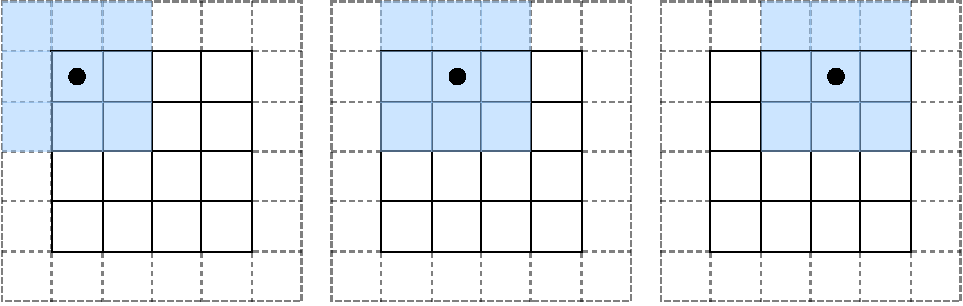
\includegraphics[width=0.8\textwidth]{figures/Image_processing_essentials.drawio.pdf}
    \caption{The image shows the three first steps (from left to right) of a general image processing method using a structuring element that is moved along the image with a stride of one to compute new pixel values. The black dot corresponds to the origin of the structuring element. The image is padded to get a new image of the same size as the old one.}
    \label{fig:image_processing_basics}
\end{figure}

Gaussian filtering approximates the kernel as a 2D gaussian distribution to perform low-pass filtering on an image. As the structuring element is slided over the image, each of the image pixels covered by the center is a sum of products of the image intensities and the values of the structuring element. $I_s(x,y)$ be the intensities of the pixels covered by the structuring element and let $S(x,y)$ be the values of each of the elements of the structuring element, both with origin at the center. Further, let the size of the structuring element be $m\times n$, with both $m$ and $n$ restricted to being odd. Then the new pixel value at the origin is:

\begin{equation}
    I_s(0,0) = \sum_{i = -\frac{n-1}{2}}^\frac{n-1}{2} \sum_{j = -\frac{m-1}{2}}^\frac{m-1}{2} I_s(i,j) \times S(i,j)
    \label{eq:gaussian_blur}
\end{equation}

The four basic morphological operators are erosion, dilation, closing, and opening, where the two latter are a combination of the first operations. In contrast to Gaussian filtering, the morphological operators are used in binary images but utilize the same sliding structuring element technique. As the image, the structuring element does also have binary values. If we again restrict the structuring element to be of odd width and height, the erosion is defined as: 

\begin{equation}
    \begin{split}
        I_s(0,0) = \prod_{i = -\frac{n-1}{2}}^\frac{n-1}{2} \prod_{j = -\frac{m-1}{2}}^\frac{m-1}{2} f(i,j) \\
        f(x,y) = 
        \begin{cases}
        I_s(x,y) & S(x,y) \neq 0 \\
        1 & otherwise
        \end{cases}
    \end{split}
    \label{eq:erosion}
\end{equation}

and the dilation as:

\begin{equation}
    I_s(0,0) = min(1, \sum_{i = -\frac{n-1}{2}}^\frac{n-1}{2} \sum_{j = -\frac{m-1}{2}}^\frac{m-1}{2} I_s(i,j) \times S(i,j))
    \label{eq:dialation}
\end{equation}

The effect of an erosion operation is that all objects are shrunk, and small objects are removed. On the other hand, the effect of dilation is that all objects are thickened, and holes in objects are filled. the effects of removing small objects and filling holes help generate consistent landmarks. However, the side effect of shrinking and thickening objects are unwanted. A dilation and erosion operation is combined to revert the side effects, and the new operations are called opening and closing. An opening operation is an erosion followed by a dilation, effectively removing small objects from the image. Closing is a dilation followed by erosion, removing holes in the image. 



% \subsubsection{Detecting shadows and echoes in sonar scan lines}

% Finding signal peaks and the width and prominence of the peaks are essential metrics in 1D signal processing. 

% \subsubsection{1D landmark detection}

% 1D landmark detection does the detection in the 1D scan lines, for example, by finding peaks and valleys in the scan line corresponding to echoes and shadow, respectively.

% \subsubsection{2D landmark detection}

% 2D landmark detection works in a 2D sonar image and uses techniques such as intensity thresholding, edge detection, and general image processing.

% \subsection{Landmark detection using deep learning}

% % This is not part of the introduction, just old notes.

% \subsection{Autonomous underwater vehicles}

% AUVs depend upon dead reckoning for navigation because of the lack of global position measurements from, for example, GNSS.
% % Avslutt avsnittet med å si at SLAM er state of the art etc og pek videre på neste subsection.

% \subsection{Simultaneously Localization and Mapping}

% SLAM is the state-of-the-art framework for robot navigation and localization.

% Feature-based or indirect SLAM uses features or landmarks to help the robot navigate.
% % Avslutt med at landmarks finnes gjennom sensoren som er farkostens "øyne" og for AUVer er det veldig typisk en sonar. 

% \subsection{Sonar}

% A sonar is a sensor that sends out acoustic pulses and measures the intensity of the echo return, and in such a way, can provide a representation of the surroundings.

% Under the supervision of  Damiano  Varagnolo and  Simon  Andreas  Hagen  Hoff, Bjørnar Reitan Hogstad has developed a sonar processing pipeline that forms the basis for this project. (Describe earlier work)

% \subsection{Landmark Detection}

% A landmark detector that can robustly detect landmarks in the seabed over various environments is needed to enable feature-based SLAM.





